% Chapter 1

\chapter{Introducción general} % Main chapter title
En este capítulo se describe la motivación del trabajo y sus objetivos, con una breve explicación sobre mediciones eléctricas digitales, que es un concepto clave en este trabajo.


\label{Chapter1} % For referencing the chapter elsewhere, use \ref{Chapter1} 
%\label{IntroGeneral}

%----------------------------------------------------------------------------------------

% Define some commands to keep the formatting separated from the content 
\newcommand{\keyword}[1]{\textbf{#1}}
\newcommand{\tabhead}[1]{\textbf{#1}}
\newcommand{\code}[1]{\texttt{#1}}
\newcommand{\file}[1]{\texttt{\bfseries#1}}
\newcommand{\option}[1]{\texttt{\itshape#1}}
\newcommand{\grados}{$^{\circ}$}

%----------------------------------------------------------------------------------------

%\section{Introducción}

%----------------------------------------------------------------------------------------
\section{Descripción general del trabajo y conceptos clave}

El trabajo desarrollado consiste en un sistema para medir potencia eléctrica. El trabajo fue desarrollado para SERVAIND S.A. que es una empresa privada localizada en Argentina  \citep{Servaind}.



\section{Medición de potencia eléctrica}

%Existe un gran número de magnitudes en el campo de la ingeniería que necesitan ser medidas o expresadas en el trabajo diario. Esto incluye cantidades físicas, mecánicas y eléctricas \citep{book:1689974}. 

%La potencia eléctrica es de interés en diversos ámbitos.

%La adquisición de datos o adquisición de señales consiste en la toma de muestras del mundo real (sistema analógico) para generar datos que puedan ser manipulados por un ordenador u otros dispositivos electrónicos (sistema digital). Se requiere una etapa de acondicionamiento, que adecua la señal a niveles compatibles con el elemento que hace la transformación a señal digital \cite{NIDataAdquisition}.

%Un convertidor de señal analógica a digital (ADC) es un dispositivo electrónico capaz de convertir una señal analógica, ya sea de tensión o corriente, en una señal digital mediante un cuantificador y codificador.

%Existen diversos métodos para la conversión de señal analógica a digital como el método de aproximaciones sucesivas, la conversión directa, la de comparación rampa, la conversación por integración y la de sigma-delta \cite{Conversores}.

%\subsection{Mediciones eléctricas digitales}

La mayoría de los medidores electrónicos digitalizan las variables medidas vía un ADC sigma-delta  de alta resolución. La técnica de diseño de estos medidores digitales está influenciada por tres grandes factores: el costo, la eficiencia y el tamaño. Mientras que el costo se ve influenciado por la capacidad de compra del cliente, la eficiencia y el tamaño se encuentran sujetos a estándares como por ejemplo el IEC-62052-11 establecido por la IEC (\textit{International Electrotechnical Commission}) \cite{articleDM}.

%IEC-62052-11
%Electricity metering equipment (AC) –
%General requirements, tests and test conditions –
%Part 11:
%Metering equipment 

\begin{figure}[h]
	\centering
	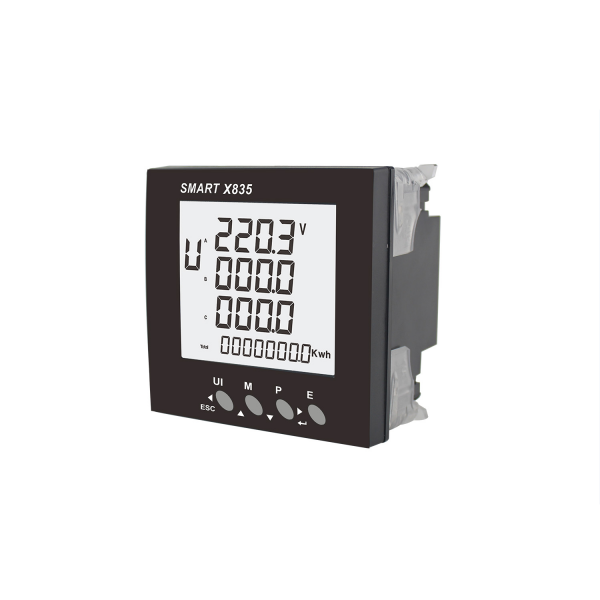
\includegraphics[width=55mm,keepaspectratio]{Figures/3931_1.png}
	\caption{Medidor electrónico comercial\protect\footnotemark .}
	\label{fig:texmaker}
\end{figure}

\footnotetext{\url{https://www.smartprocess.co.uk/}}

La exactitud del medidor eléctrico digital depende de la precisión del circuito de entrada analógica, la del conversor analógico-digital y la de los cálculos digitales \citep{Hribik2004DigitalPA}.

Los convertidores analógico-digitales basados en la modulación sigma-delta son económicamente viables para convertidores de alta resolución (mayores que 12 bits), por lo que son  usados en el circuito integrado de procesadores de señales.

%La modulación sigma-delta fue introducida en 1962 y no ganaría importancia hasta recientes desarrollos en tecnologías VLSI (integración a escala muy grande) que proveen fines prácticos para implementar complejos circuitos de procesamiento de señales \citep{book:28601}.


\section{Estructura del trabajo}

\label{sec:structdescript1}
Inicialmente se realizó un plan de trabajo \cite{planTrabajo} donde se plantea cómo se afronta el problema y el modo en que se lo resolverá. El proyecto propuesto consta de dos partes principales: hardware y software.

Para el hardware se planteó un diagrama de bloques que sirvió de guía al realizar el circuito esquemático, que puede verse en la figura \ref{fig:bloquess1}. El diagrama planteó dos sectores, uno de procesamiento y otro de medición que se encontraran aislados.

\begin{figure}[h]
	\centering
	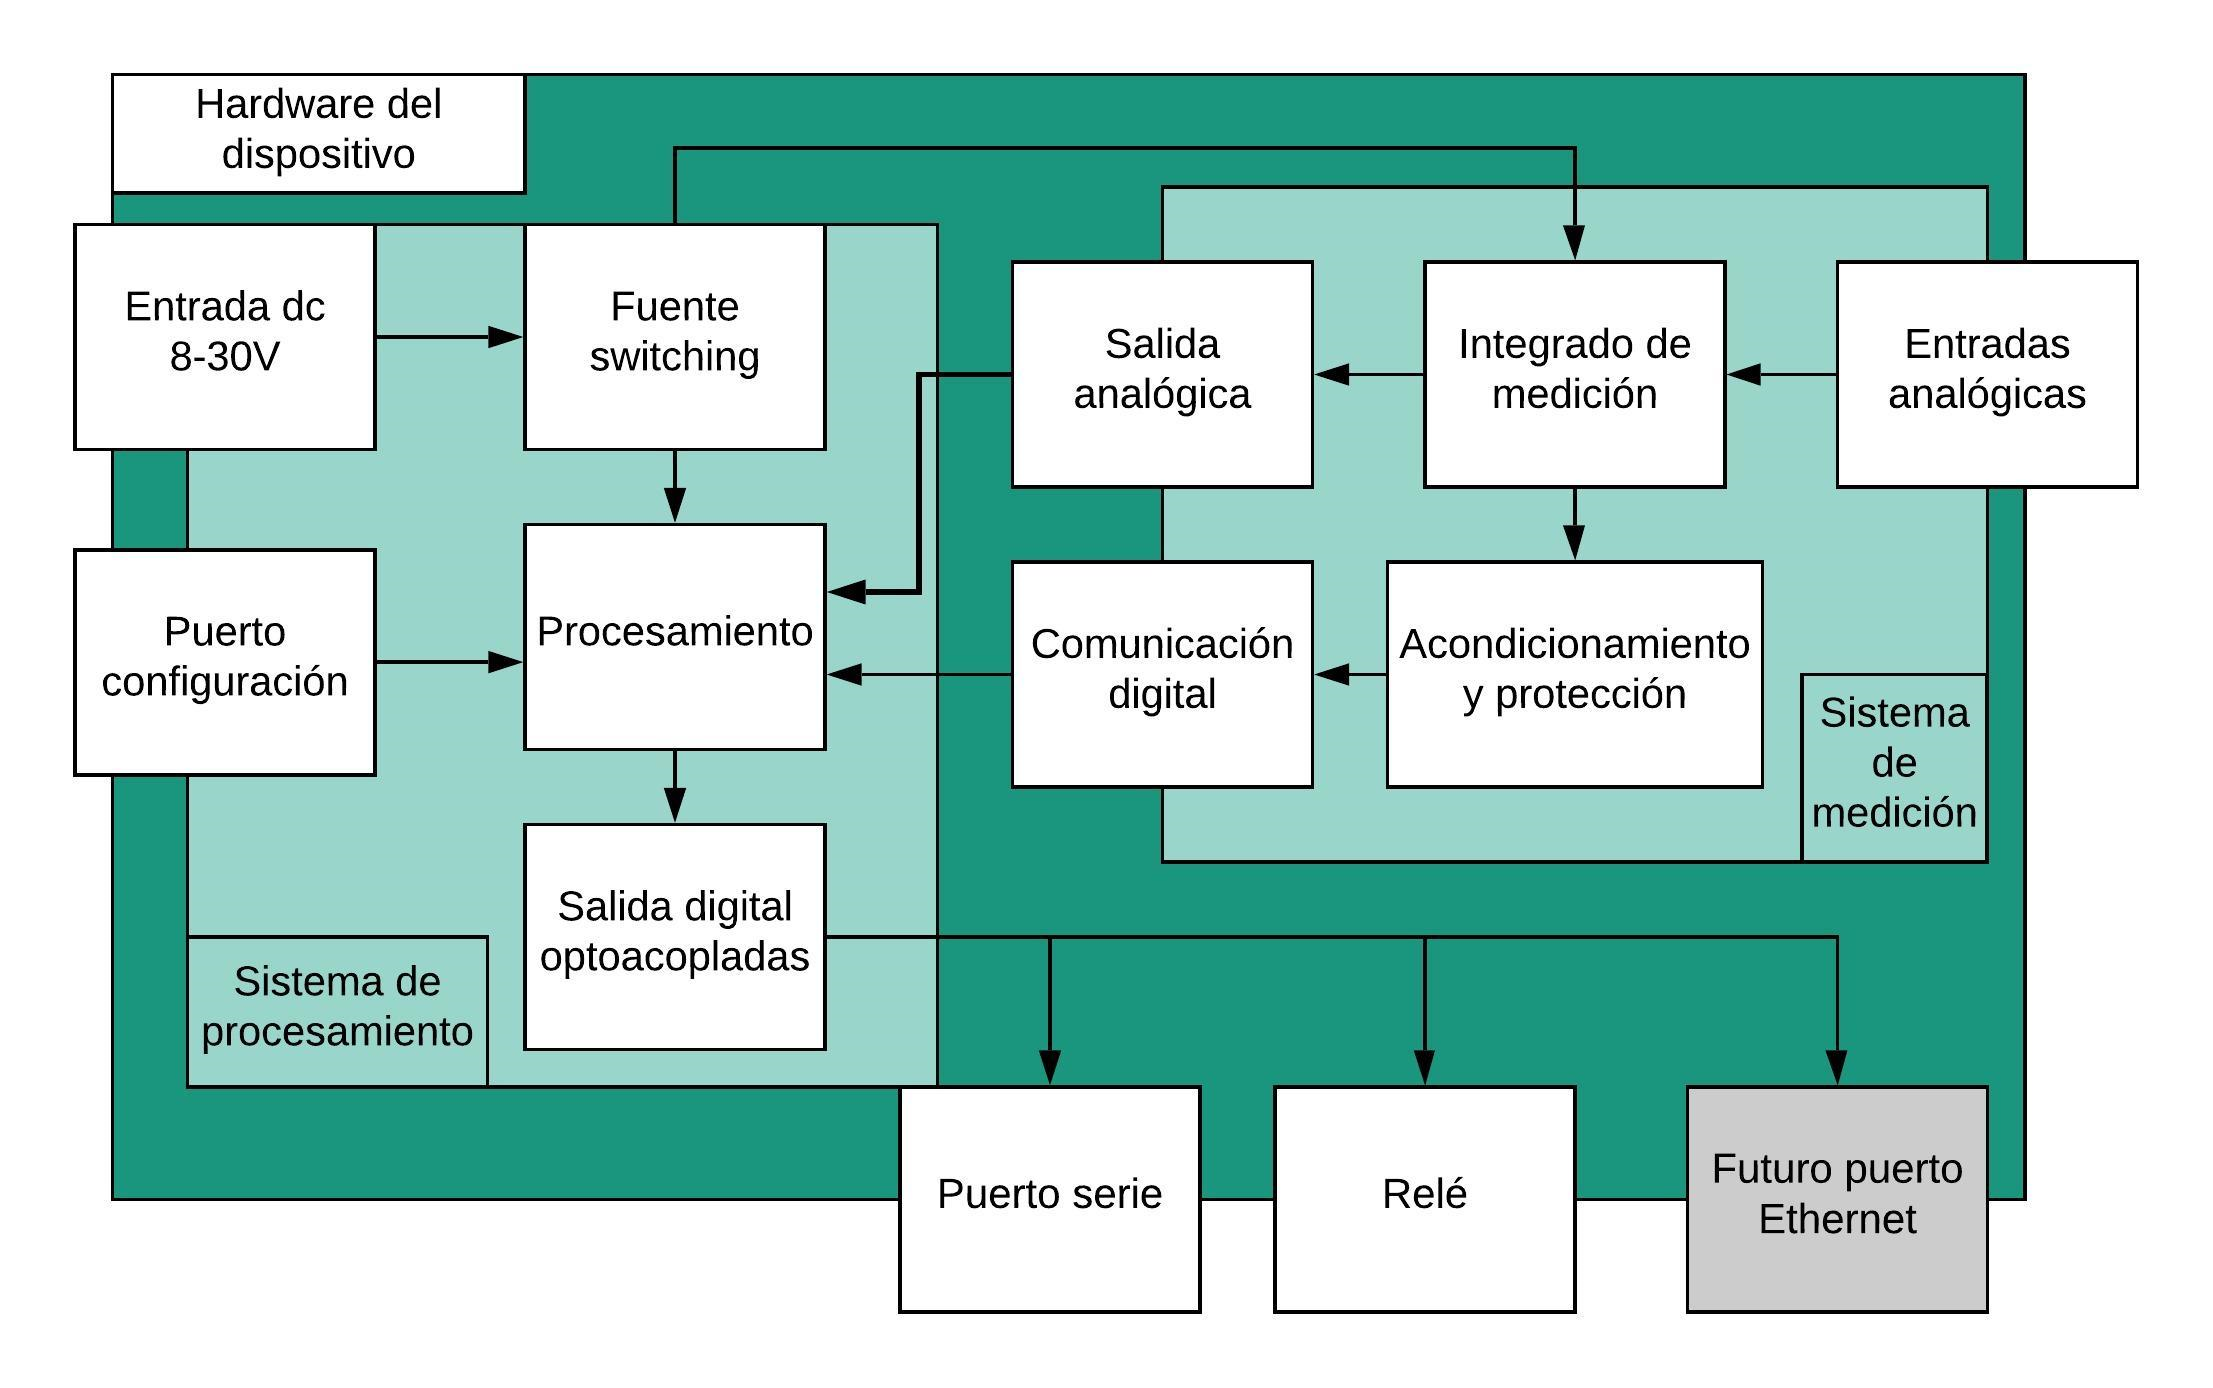
\includegraphics[width=\textwidth,keepaspectratio]{Figures/concepto.png}
	\caption{Diagrama en bloques del hardware.}
	\label{fig:bloquess1}
\end{figure}

El diagrama presupone que se usará una entrada de alimentación de corriente continua de 8 a 30 V conectado a una fuente \textit{switching}, donde alimentará tanto al procesamiento como a la medición.

En el subsistema \textquotedblleft sistema de procesamiento\textquotedblright \ de la figura \ref{fig:bloquess1}, se estableció que el hardware contaría con un puerto de configuración y varias salidas optoacopladas. Se planteó que estas salidas fuesen un relé, un puerto serie y un puerto Ethernet.

Se propuso  también que el subsitema \textquotedblleft sistema de medición\textquotedblright \ de la figura \ref{fig:bloquess1}, se conectara al sector \textquotedblleft sistema de procesamiento\textquotedblright \ por una comunicación digital aislada y también por una salida analógica. 

%Además se indicó que la medición tendría varias entradas analógicas, pero no fueron especificadas.

En cuanto al software, se estableció que sea el necesario para lograr el testeo de las partes del hardware y la verificación de los requerimientos, por lo que debía manejar correctamente todos los integrados que fueran a estar embebidos en el circuito del dispositivo y manejar todos los protocolos definidos en los requisitos.

En la primera parte del trabajo se armó la electrónica del prototipo y el software se fue construyendo  para demostrar el funcionamiento del hardware. 

Una vez finalizado el armado del hardware se procedió a una segunda parte del desarrollo del software, donde debía además de comunicarse con diferentes protocolos, ser capaz de realizar diferentes configuraciones del dispositivo según requiera el usuario.


\section{Motivación}

En la actualidad se pueden encontrar en el mercado internacional múltiples módulos electrónicos de bajo costo con puertos de comunicación para la medición de energía eléctrica. Asimismo, existen medidores digitales de energía de diferentes marcas para diferentes entornos, lo que permite pensar que un dispositivo similar podría ser fabricado en la Argentina.

Los módulos de medición pueden servir para apoyar a sistemas de seguridad. Estos actuarían como un método preventivo de fallas, dado que los parámetros de consumo dan una idea del estado de las máquinas eléctricas.  

El módulo de la figura \ref{fig:pzem04} es un medidor de energía que se comunica mediante una interfaz serie universal \cite{modulopezetaeme}. El módulo fue usado por el autor en una experiencia previa, en la cual varias copias de este se instalaron en un local comercial. Con el conjunto de estos módulos se logró medir el consumo de los electrodomésticos presentes en el lugar de trabajo. Gracias a su implementación se detectaron fallas en algunas máquinas. Además se observó el comportamiento del aparato eléctrico de mayor consumo del local que es la cámara frigorífica (que representa más del 25\% del consumo total), cuyo comportamiento puede verse en la figura \ref{fig:graficoW}.  

\begin{figure}[h]
	\centering
	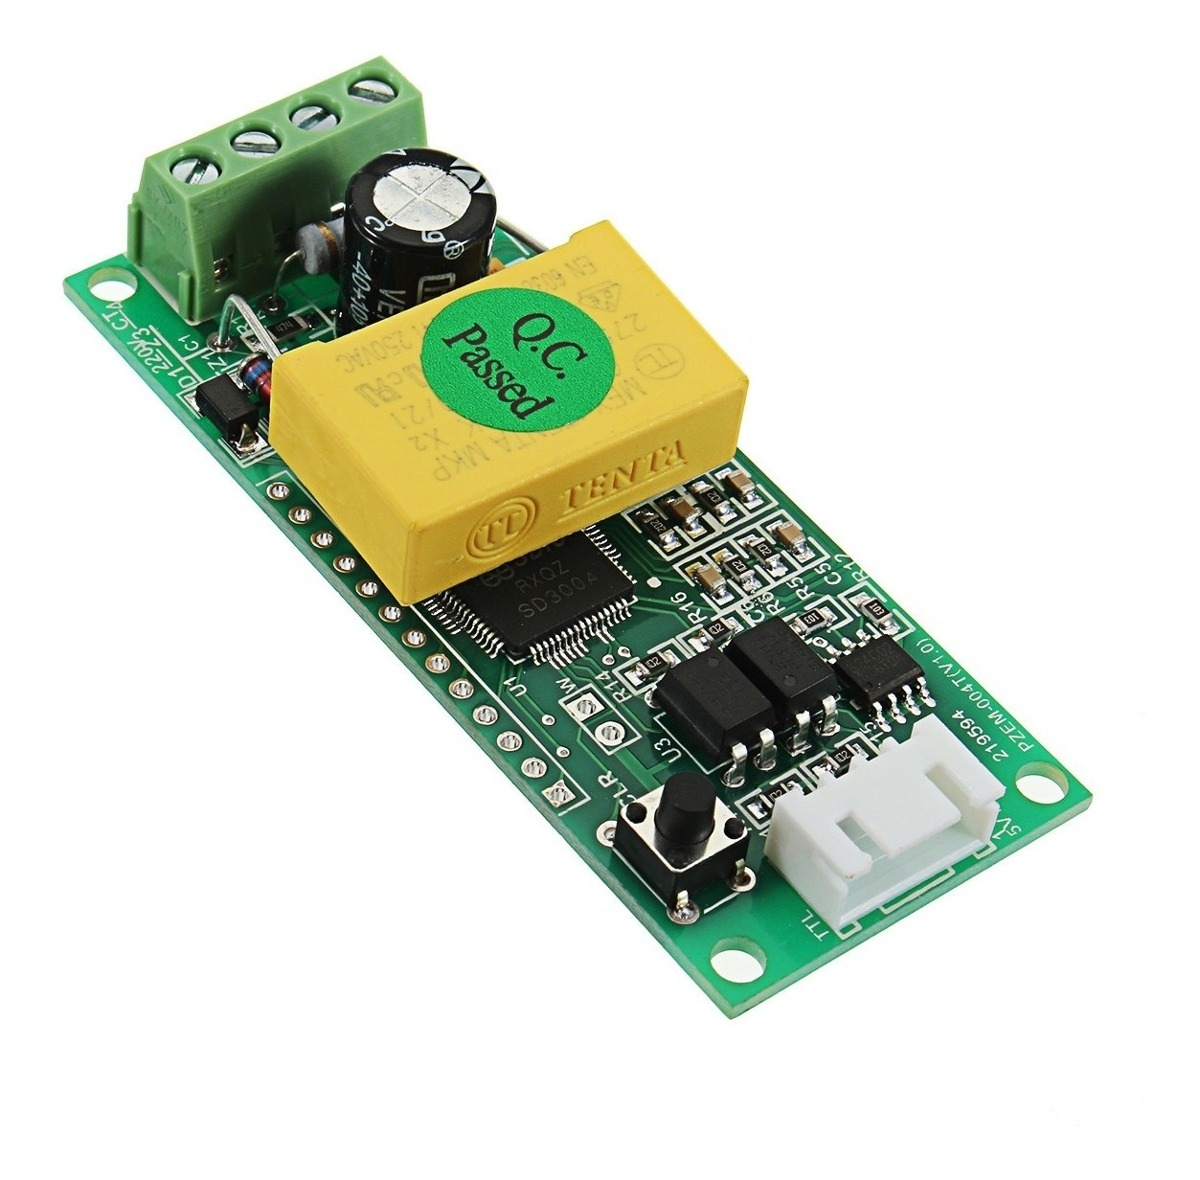
\includegraphics[width=80mm,keepaspectratio]{Figures/pzeem004.jpg}
	\caption{Módulo de medición de energía eléctrica con comunicación serie universal\protect\footnotemark .}
	\label{fig:pzem04}
\end{figure}

\footnotetext{\url{ https://peacefair.es.aliexpress.com/store/1773456}}

Estos módulos se consiguen únicamente en el mercado internacional de modo que hay que importarlos, lo que presenta una barrera para una herramienta de mucha utilidad.

\begin{figure}[!htb]
	\centering
	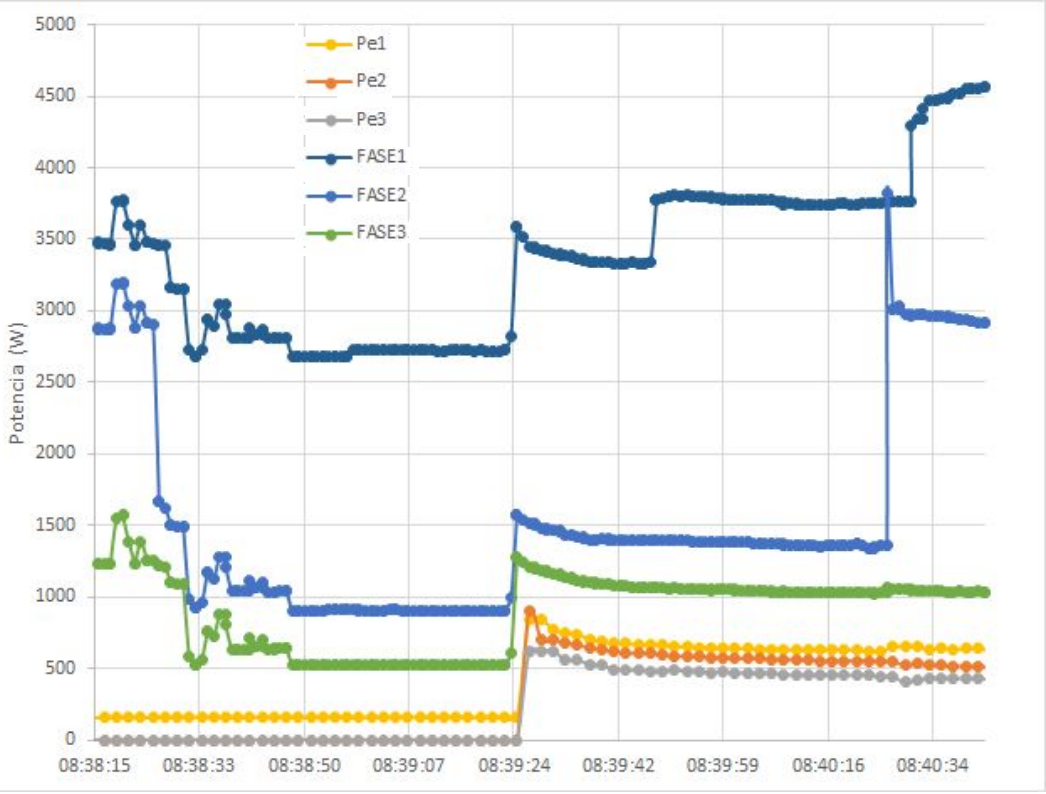
\includegraphics[width=120mm,keepaspectratio]{Figures/potencia_ej.png}
	\caption{Gráfico de medición de potencia que muestra el encendido del motor trifásico de compresión de un frigorífico.}
	\label{fig:graficoW}
\end{figure}

Las curvas de la figura \ref{fig:graficoW} sirvieron para tener una idea más clara del funcionamiento del encendido de la cámara frigorífica y saber el costo energético que implica. Además gracias a los datos recabados se lograron detectar el mal funcionamiento en otros equipos eléctricos de refrigeración.
 
Desde el punto de vista de SERVAIND S.A., el trabajo se planteó ante la necesidad de cuantificar consumos energéticos de procesos industriales para supervisar la alimentación de equipos de control o de medición. También como una alternativa a un producto anterior que solo medía consumos de corriente continua. En suma, la necesidad de hacer uso de la herramienta y poseer los medios necesarios para fabricar la electrónica de manera local  impulsaron el trabajo realizado.



\section{Requerimientos del trabajo}
\label{sec:cap2parte2}
Los requerimientos fueron elaborados a partir de un documento enviado por el equipo de desarrollo de la empresa SERVAIND S.A. y se resumen en la siguiente lista:

\begin{itemize}
\item Grupo de requerimientos referidos a medición de potencia del equipo:
\begin{enumerate}
\item El dispositivo debe ser capaz de realizar la medición de tensión alterna de una línea monofásica de baja tensión de Argentina, entrada de medición para 220 V o 380 V con una tolerancia de +/-15\%.
\item El dispositivo debe ser capaz de realizar la medición de corriente alterna de una línea monofásica de baja tensión de Argentina, hasta 5 A.
\item El dispositivo debe ser capaz de realizar la medición de potencia eléctrica activa de una línea monofásica de baja tensión de Argentina, hasta 4000 W.
\item El sistema de medición que se utiliza para las mediciones debe ser aislado de la salida de comunicaciones del puerto serie.
\end{enumerate}

\item Grupo de requerimientos referidos a interfaces de comunicación:
\begin{enumerate}
\setcounter{enumi}{4}
\item El dispositivo debe realizar las comunicaciones a través de protocolos RS485 y RS232.
\item El dispositivo debe tener en su diseño espacio para una posible modificación a futuro en la que se incluya una interfaz Ethernet a través de una entrada para rj45.
\end{enumerate}

\item Grupo de requerimientos referidos a diseño del circuito eléctrico:
\begin{enumerate}
\setcounter{enumi}{6}
\item El dispositivo debe alimentarse con tensión continua que debe ser inferior a 30 V y superior a 12 V.
\item El dispositivo debe poseer como microcontrolador principal MSP430F2418.
\item El dispositivo debe implementar protecciones contra sobretensión en salida y entradas.
\item El dispositivo debe tener un relé para realizar un corte por corriente.
\end{enumerate}

\item Grupo de requerimientos referidos a diseño  de impresión del circuito:
\begin{enumerate}
\setcounter{enumi}{10}
\item El tipo de soldado debe ser por refusión en la cara superior del circuito impreso.

\item El tipo de soldado debe ser por ola en la cara inferior del circuito impreso.
\end{enumerate}
\end{itemize}


\section{Objetivos y alcance}

\subsection{Objetivos del desarrollo}

El objetivo del trabajo fue el desarrollo de un dispositivo de medición basado en un microcontrolador de la familia MSP430 en conjunto con un ADC SOC (\textit{system on chip}). Se pretendió lograr un dispositivo comercial similar a aquellos elaborados anteriormente por la empresa privada, por lo que las dimensiones del PCB (\textit{Printed Circuit Board}) deberán ajustarse a las utilizadas por las carcasas estándar que utiliza la empresa, como puede verse en la figura \ref{fig:disp_emp}.

\begin{figure}[!h]
	\centering
	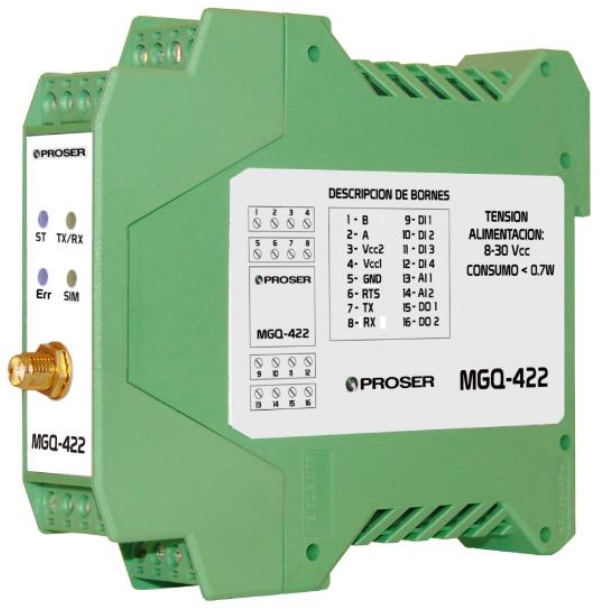
\includegraphics[width=80mm,keepaspectratio]{Figures/dispositivo_empresa.png}
	\caption{Ejemplo de dispositivo fabricado por la empresa SERVAIND\protect\footnotemark}
	\label{fig:disp_emp}
\end{figure}


\footnotetext{Imagen tomada de \url{http://www.proser.com.ar/}}

Además, se esperaba que el firmware manejara protocolo Modbus y comunicara las variables medidas a través de los puertos de comunicación. Físicamente se estableció que el dispositivo fuera capaz de comunicar por puertos serie RS-232 y RS-485, y que este pudiera funcionar en un ambiente industrial (el dispositivo tendría que ser robusto).


\subsection{Alcances}


%----------------------------------------------------------------------------------------

El trabajo abarcó el planteo, diseño y fabricación de un PCB. Asimismo, incluyó la selección de componentes, la elaboración del esquemático de conexiones lógicas y la elaboración del PCB y su diseño para la fabricación. Además se debió elaborar un prototipo y realizar testeos.

También se esperaba realizar un firmware para el funcionamiento del dispositivo, teniendo en cuenta que el software debía incluir métodos de configuración para un futuro usuario.
